\chapter{Machine Learning} \label{chp:machinelearning}
\epigraph{In the early 1990's we were working with machine learning all the time, but back then we called it pattern recognition and regression.}{Prof. Anne Solberg, UiO}
\begin{figure}[H]
	\centering
	\includegraphics[scale=0.25]{Images/brain.png}
	\caption{Artificial neural networks are inspired by neural networks in the brain.\\ © Copyright trzcacak.rs.}
\end{figure}

The use of the term \textit{machine learning} has exploded over the past years, and sometimes it sounds like it is a totally new field. However, the truth is that many of the methods are relatively old, where for instance \textit{linear regression} was known early in the 19th century \cite{legendre_nouvelles_1805, gauss_theoria_1809}. Those methods have just recently been taken under the machine learning umbrella, which is one of the reasons why the term is used more frequently than before. Another important contributor to the booming popularity is the dramatically improvement of a majority of machine learning algorithms. We will come back to this, but before that we will make an attempt defining the term machine learning.

Unlike traditional algorithms, machine learning algorithms are not told what to do explicitly, but they use optimization tools to find patterns in a data set with or without prior knowledge. Based on this, we land at the following definition:

\begin{shadequote}{}
	Machine learning is the science of getting computers to act without being explicitly programmed.
\end{shadequote}

As a consequence, we often do not know exactly what the algorithm does and why it behaves as is does. Because of this behavior and the fact that artificial neural networks are inspired by the human brain, the processing is often called artificial intelligence. In our search for a technique to solve quantum mechanical problems where less physical intuition is needed, machine learning appears as a natural tool.

Especially the artificial neural networks have experienced a significant progress over the past decade, which can be attributed to an array of innovations. Most notably, the convolutional neural network (CNN) \textbf{AlexNet}  managed to increase the top-5 test error rate of image recognition with a remarkable 11.1\% compared to the second best back in 2012 \cite{krizhevsky_imagenet_2012}! Today, the CNNs have been further improved, and they are even able to beat humans in recognizing images! \cite{alom_history_2018} Also voice recognition algorithms have lately been revolutionized, thanks to recurrent neural networks (RNNs), and especially long short-term memory (LSTM) networks. Their ability to recognize sequential (time-dependent) data made the technology good enough for an entry to millions of peoples everyday-life through services such as \textbf{Google Translate} \cite{wu_googles_2016}, Apple's \textbf{Siri} \cite{smith_ios_2016} and \textbf{Amazon Alexa} \cite{noauthor_bringing_nodate}. It is also interesting to see how machine learning has made computers eminent tacticians using reinforcement learning. The \textbf{Google DeepMind} developed program \textbf{AlphaGo} demonstrated this by beating the 9-dan professional L. Sedol in the board game Go \cite{noauthor_alphago_nodate}, before an improved version, \textbf{AlphaZero}, beat the at that time highest rated chess computer, \textbf{StockFish}, plying chess. \cite{klein_mikeklein_googles_nodate} Both these scenarios were unbelievable just a couple of decades ago.

Even though all these branches are both exciting and promising, they will not be discussed further in this work, since they will simply not work for our purposes. The reason is that they initially require a data set with known outputs in order to be trained, they obey so-called \textit{supervised} learning. Instead, we rely on \textit{unsupervised} learning, which has the task of finding patterns in the data and is therefore not in need for known outputs. However, we will discuss some simpler supervised learning algorithms as an introduction and a motivation for the unsupervised learning section.

\section{Supervised learning}
As hinted above, in machine learning we want to fit a model to a data set in the best possible way. In supervised learning, we have prior knowledge about what kind of results the model should give in some specific cases, which we can use to train our model. After training, we want the model to
\begin{enumerate}
	\item be able to reproduce the \textit{targets} (the prior known results)
	\item be able to fit future observations.
\end{enumerate}
In this section we will take a closer look at how to find a model which satisfies both these goals. If the first one is satisfied, the second is not necessarily satisfied. Let us first look at polynomial regression. 

\subsection{Polynomial regression}
Polynomial regression is perhaps the most intuitive example on this, where we want to find the line that fits some data points in the best possible way. In two dimensions, the data set consists of some $n$ number of x- and y coordinates,
\begin{align*}
\bs{x}&=(x_1,x_2,\hdots,x_n)\\
\bs{y}&=(y_1,y_2,\hdots,y_n)
\end{align*}
which we for instance could try to fit to a second order polynomial,
\begin{equation}
f(x)=ax^2+bx+c,
\end{equation}
where the parameters $a$, $b$ and $c$ are our estimators. The polynomial is now our model. By inserting the $x$-values into the polynomial, we obtain a set of equations
\begin{equation}
\mqty{
	\tilde{y}_1&=&ax_1^2&+&bx_1&+&c\\
	\tilde{y}_2&=&ax_2^2&+&bx_2&+&c\\
	\vdots&&\vdots&&\vdots&&\vdots\\
	\tilde{y}_n&=&ax_n^2&+&bx_n&+&c
}
\label{eq:lineareqs}
\end{equation}
where $\tilde{y}_i=f(x_i)$ is the $y$-value of the polynomial at $x=x_i$. What we want to do is to determine the estimators $a$, $b$ and $c$ such that the mean squared error (MSE) of all these equations is minimized,
\begin{equation}
\min_{a,b,c}\frac{1}{n}\sum_{i=0}^{n-1}(y_i-f(x_i;a,b,c))^2.
\end{equation}
There are several ways to do this, but they all are based on the \textit{cost function} (also called the loss function), which can simply be defined as the MSE,
\begin{empheq}[box={\mybluebox[5pt]}]{equation}
\mathcal{C}(a,b,c)=\frac{1}{n}\sum_{i=0}^{n-1}\Big(y_i-(ax_i^2+bx_i+c)\Big)^2,
\end{empheq}
and which we seek to minimize. Before we start minimizing this, we will introduce a more general notation, where the estimators are collected in a column vector 
\begin{equation*}
\bs{\theta}=(a,b,c)^T
\end{equation*}
and the $x_i^j$'s also are collected in a row vector
\begin{equation*}
\bs{X}_i=(x_i^2, x_i, 1).
\end{equation*}
Using this, the cost function can be written as
\begin{align}
\mathcal{C}(\bs{\theta})&=\frac{1}{n}\sum_{i=0}^{n-1}\Big(y_i-\sum_{j=0}^2X_{ij}\theta_j\Big)^2\notag\\
&=\frac{1}{n}\sum_{i=0}^{n-1}\Big(y_i-\bs{X}_i\bs{\theta}\Big)^2\label{eq:costols}\\
&=\frac{1}{n}(\bs{y}-\bs{X}\bs{\theta})^T(\bs{y}-\bs{X}\bs{\theta})\notag
\end{align}
where we in the last step have collected all the vectors $\bs{X}_i$ in a matrix. As the minimum of the cost function with respect to a estimator $\theta_j$ is found when the derivative is zero, we need to solve
\begin{align*}
\frac{\partial \mathcal{C}(\bs{\theta})}{\partial\theta_j} &=\frac{\partial}{\partial\theta_j}\bigg(\frac{1}{n}\sum_{i=0}^{n-1}\Big(y_i-\sum_{j=0}^2X_{ij}\theta_j\Big)^2\bigg)\notag\label{eq:gh}\\
&=\frac{2}{n}\sum_{i=0}^{n-1}X_{ij}\Big(y_i-\sum_{j=0}^2X_{ij}\theta_j\Big)=0.
\end{align*}
We can go further and write it on matrix-vector form as
\begin{equation*}
\frac{\partial \mathcal{C}(\bs{\theta})}{\partial\bs{\theta}}=\frac{2}{n}\bs{X}^T(\bs{y}-\bs{X}\bs{\theta})=0
\end{equation*}
where differentiating with respect to a vector here means that each component is $\partial\mathcal{C(\bs{\theta})}/\partial\theta_j$. This is satisfied if
\begin{equation}
\bs{\theta}=(\bs{X}^T\bs{X})^{-1}\bs{X}^T\bs{y}
\label{eq:polynomialestimators}
\end{equation}
which is the equation we seek to solve to find the best fitting polynomial. Before we proceed to the general case, let us have a quick look at an example.

\subsubsection{Example} \label{sec:example}
In this example, we will see how we in practice fit a polynomial to a data set. Suppose we have a tiny data set consisting of 10 points on a plane
\begin{align}
\bs{x}&=(1,2,4,6,7,9,10,11,13,16)\notag\\
\bs{y}&=(15,30,50,60,65,63,60,55,40,0)
\label{eq:datapoints}
\end{align}
to which we want to fit a polynomial of degree $p$. The data points can be seen in figure (\ref{fig:polynomials} a). The first thing we need to realize, is that in order to validate our models, we cannot use all points for the training. There is no strict rules on how much of the data set that should be used for training and validation, but at least the training data set should be larger than the validation data set. For this particular problem, we decide to leave out $\{(1,15),(9,63),(10,60)\}$ from the training, which we later will use for validation.

Furthermore, we use equation \eqref{eq:polynomialestimators} to find the best fitting first-, second- and sixth order polynomials, and obtain the functions presented in table \eqref{tab:example} with the respective training and prediction errors. The polynomials are also plotted in figure (\ref{fig:polynomials} b) together with the actual data points.

\begin{figure}
	\centering
	\subfloat[Data set]{{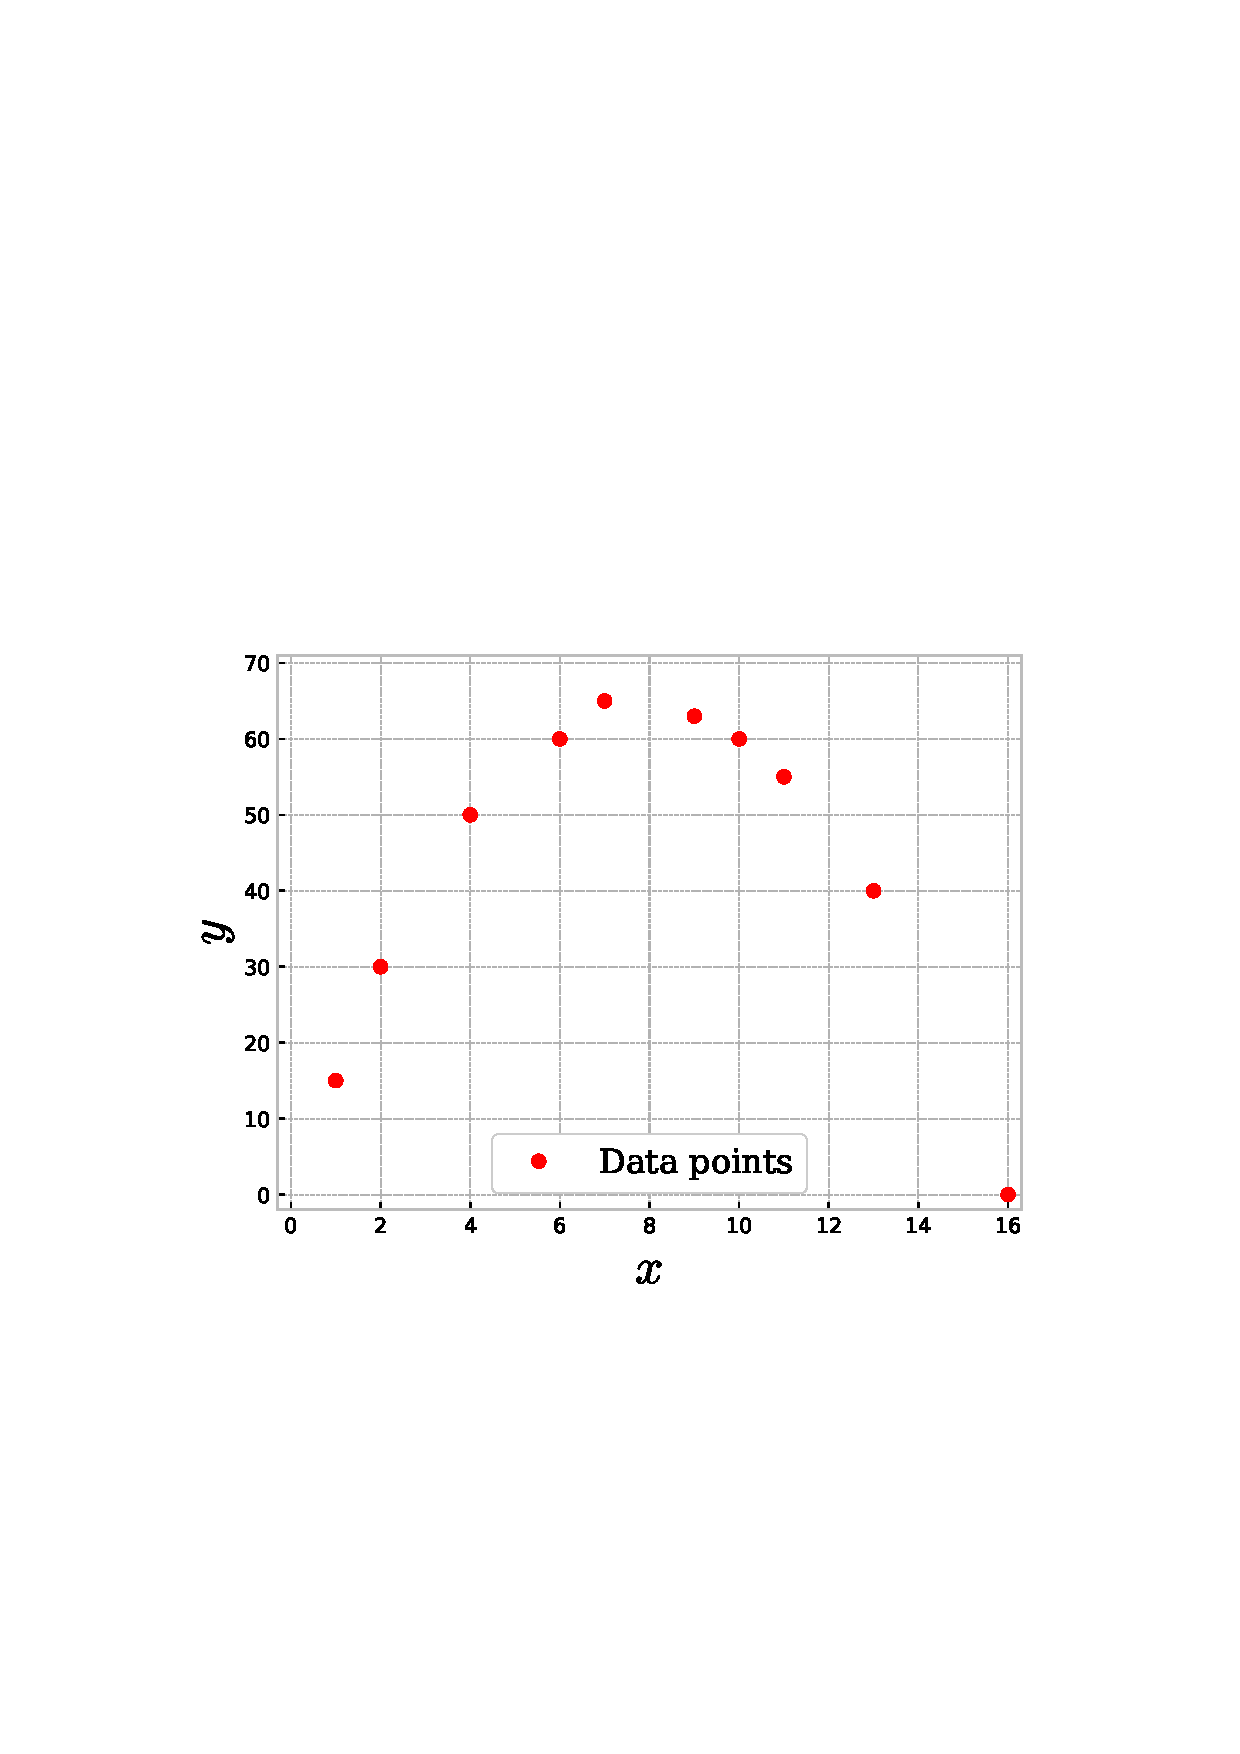
\includegraphics[width=8cm]{Images/datapoints.png}}}
	\subfloat[Data set with fitted polynomials]{{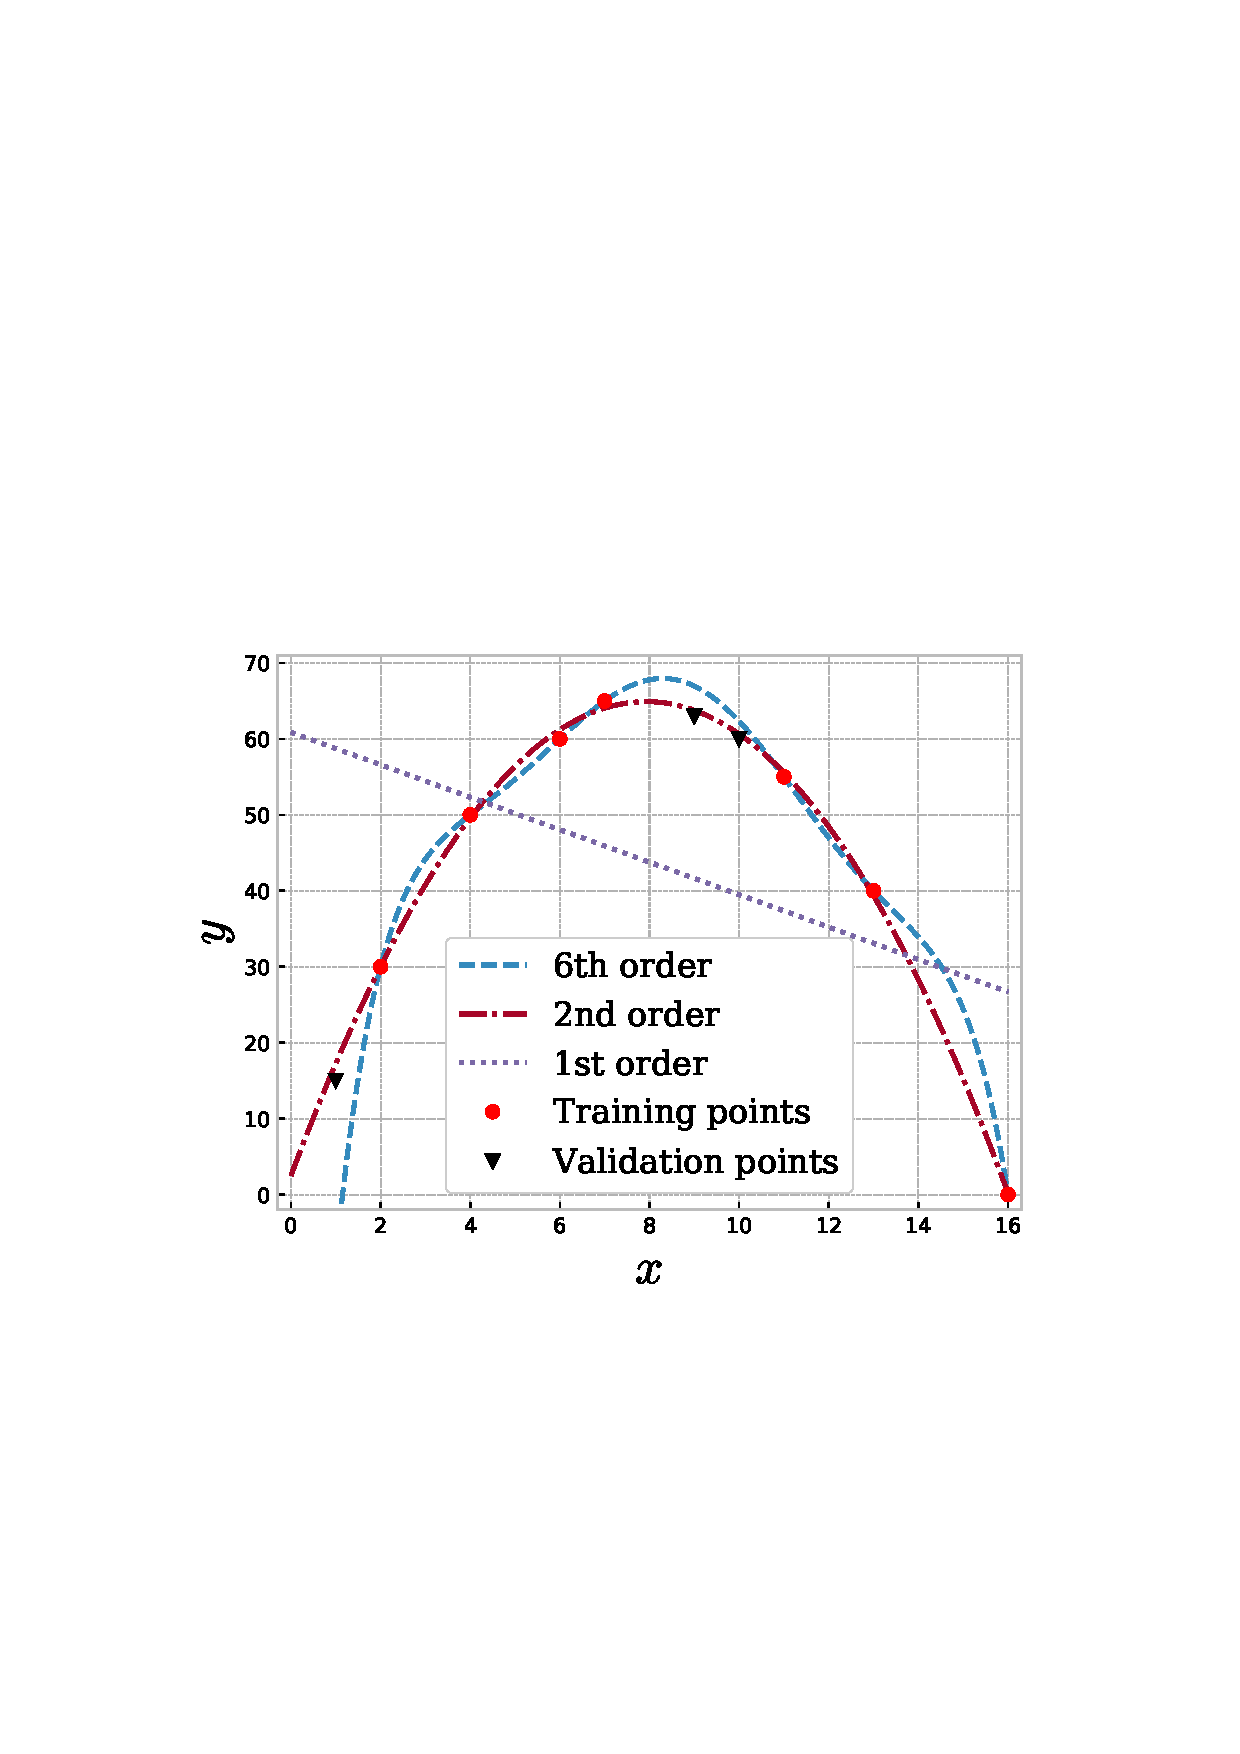
\includegraphics[width=8cm]{Images/datacurve.png} }}
	\caption{Figure (a) presents the data points given in \eqref{eq:datapoints}, while the figure (b) illustrates how a first-, second- and third order polynomial can be fitted to the training set in the best possible way.}%
	\label{fig:polynomials}
\end{figure}

\begin{table}
	\caption{Best fitting polynomials of 1st, 2nd and 6th order degree to the data set in equation \eqref{eq:datapoints}. $f(x)$ gives the actual form of the polynomial, the training error gives the MSE to the training data set and the prediction error gives the MSE to the validation set.}
	\label{tab:example}
	\begin{tabularx}{\textwidth}{llXXX} \hline\hline
		Order & \makecell{\\ \phantom{=}} & $f(x)$ & Training error & Prediction error \\ \hline \\
		
		1st && $-2.14x+60.87$ & 327.22 & 927.87 \\
		2nd && $-x^2+15.74x + 2.51$ & 0.47 & 2.04 \\
		6th && $-0.001x^6+0.04x^5-0.90x^4+9.04x^3-47.52x^2+129.74x-98.67$ & 2.54E-11 & 187.53 \\ \hline\hline
	\end{tabularx}
\end{table}

What we immediately observe, is that the more complex model (higher degree polynomial) the lower training error. In fact, the polynomial of sixth order reproduces the points perfectly. The first order polynomial is quite bad, while the second order polynomial is intermediate.

However, what really makes sense is the prediction error, and for that we can see that the sixth order polynomial performs terribly. When a model can reproduce the training set very well, but is not able to reproduce the training set, we say that it overfits the data set. This means that the model is too complex for the purpose.

On the other hand, we see that the first order polynomial has also a large prediction error, which means that it is not able to reproduce the validation set either. We say that it is underfitted, and we are in need of a more complex model.

Finally, we have the second order polynomial, which is miles ahead its competitors when it comes to the prediction error. It turns out that the second order model has an appropriate complexity, which we could have guessed just by looking at the data points.

The natural question now is \textit{"How do we find a correct model complexity?"}. The answer is that one should try various complexities and calculate the prediction error for each model. To find the prediction error precisely, the standard is to use $K$ cross-validation resampling, which tries $K$ choices of validation set to make the most use of our data. More about resampling analysis can be found in section \eqref{sec:resampling}. A deeper understanding of the prediction error will hopefully be gained in the next section, on bias-variance decomposition. 

\subsection{Bias-variance tradeoff}
Up to this point, we have skipped some important terms in the statistics behind machine learning. First, we have the \textit{bias}, which describes the best our model could do if we had an infinite amount of training data. We also have the \textit{variance}, which is a measure on the fluctuations in the predictions. In figure (\ref{fig:bias_variance} a), example on high variance low-bias and a low variance high bias models are presented. What we actually want is a low variance low-bias model, but this model is normally infeasible and we need to find the optimal tradeoff between bias and variance. This is known as the bias-variance tradeoff. 

\begin{figure}
	\centering
	\subfloat[Illustration of bias and variance]{{\includegraphics[width=8cm]{Images/bias_variance.png}}}
	\subfloat[Bias-variance trade-off]{{\includegraphics[width=8cm]{Images/bias_variance_tradeoff.png} }}
	\caption{Examples of high variance, low-bias and low variance high-bias (a) and illustration of the bias-variance trade-off (b). Figures are taken from Mehta et.al., \cite{mehta_high-bias_2019}.}%
	\label{fig:bias_variance}
\end{figure}

In figure (\ref{fig:bias_variance} b), the bias-variance tradeoff is illustrated as a function of the model complexity. We observe that the prediction error if large when the model complexity is too low, which corresponds to a low variance. This substantiates what we discussed in the example in \eqref{sec:example}, where we claimed that a too low model complexity underfits the data set. Therefore, a too low variance is associated with underfitting.

On the other side of the plot, we can see that also a too complex model causes a large prediction error, which corresponds to a low bias. As discussed before, a too complex model overfits the model, which is associated with low bias. 

To minimize the prediction error, we should therefore neither minimize the bias nor the variance. Instead, we should find the bias and variance which corresponds ot the lowest error. The prediction error can also be decomposed into bias and variance, given by
\begin{equation}
E[(y-\tilde{y})^2]=\text{bias}[\tilde{y}]^2+\sigma^2[\tilde{y}]
\end{equation}
where 
\begin{equation}
\text{bias}[\tilde{y}]=E[\tilde{y}]-y
\end{equation}
and 
\begin{equation}
\sigma^2[\tilde{y}]=E[\tilde{y}^2]-E[\tilde{y}]^2.
\end{equation}

\subsection{Linear regression}
Polynomial regression, as already discussed, is an example on a linear regression method, and was meant as motivation before we study linear regression in general. Instead of fitting a polynomials to a set of points, we can fit a general function on the form
\begin{equation}
f(x_i)=\sum_{j=0}^pX_{ij}(x_i)\theta_j
\label{eq:targets}
\end{equation}
where we have $p$ estimators $\theta_j$. The matrix $\bs{X}$ is called the \textit{design matrix}, and the case where $X_{ij}(x_i)=x_i^j$ corresponds to polynomial regression, but it can in principle be an arbitrary function of $x_i$.

The cost function for \textit{the ordinary least square regression} (OLS) case is already found in equation \eqref{eq:costols}, and we can recall it as
\begin{empheq}[box={\mybluebox[5pt]}]{equation}
	\mathcal{C}(\bs{\theta})=\sum_{i=1}^{n}\Big(y_i-\sum_{j=0}^pX_{ij}\theta_j\Big)^2,\qquad\qquad\qquad\text{OLS}
\end{empheq}
which is minimized when
\begin{equation}
\bs{\theta}=(\bs{X}^T\bs{X})^{-1}\bs{X}^T\bs{y}.
\label{eq:ols}
\end{equation}

To solve this equation, we need to find the inverse of the matrix $\bs{X}^T\bs{X}$, which is typically done by \textit{lower-upper} decomposition (LU) or \textit{singular values decomposition} (SVD). Quite often when we deal with large data sets, the matrix above is singular, which means that the determinant of the matrix is zero. In those cases, we cannot find the inverse, and LU decomposition does not work. Fortunately, SVD \textit{always} works, and in cases where the matrix is singular, it turns out to be a good idea.

\subsubsection{Singular value decomposition}
Singular value decomposition is a method which decomposes a matrix into a product of three matrices, written as
\begin{equation}
\bs{X}=\bs{U}\bs{\Sigma}\bs{V}^T.
\end{equation}
This might sounds like a bad idea, but especially for singular matrices this often makes life easier. The reason for this, is that only $\Sigma$ is singular after the decomposition. For our case, we can thus write the matrix $\bs{X}^T\bs{X}$ as 
\begin{equation}
\bs{X}^T\bs{X}=\bs{V}\bs{\Sigma}^T\bs{\Sigma}\bs{V}^T=\bs{V}\bs{D}\bs{V}^T
\end{equation}
which is non-singular. By multiplying with $\bs{V}$ on the right-hand-side, we obtain 
\begin{equation}
(\bs{X}^T\bs{X})\bs{V}=\bs{V}\bs{D}
\end{equation}
and similarly
\begin{equation}
(\bs{X}\bs{X}^T)\bs{U}=\bs{U}\bs{D}
\end{equation}
when transposing the matrix. Using those expressions, one can show that
\begin{equation}
\bs{X}\bs{\theta}=\bs{U}\bs{U}^T\bs{y}.
\end{equation}

\subsubsection{Ridge regression}
So, how can we avoid non-singular values in our matrix $\bs{X}^T\bs{X}$? We can remove them by introduce a penalty $\lambda$ to ensure that all the diagonal values are non-zero, which can be accomplished by adding a small value to all diagonal elements. Doing this, all diagonal elements will get a non-zero value and the matrix is guaranteed to be non-singular. Still using the matrix-vector form, this can be written as 
\begin{equation}
\bs{\theta}=(\bs{X}^T\bs{X}+\lambda\bs{I})^{-1}\bs{X}^T\bs{y}
\end{equation}
where $\bs{I}$ is the identity matrix. The penalty $\lambda$ is also a \textit{hyper parameter}, which is a parameter that is set before the training begins, in contrast to the estimators which are determined throughout training. This method is called Ridge regression, and has a cost function given by 
\begin{empheq}[box={\mybluebox[5pt]}]{equation}
	\mathcal{C}(\bs{\theta})=\sum_{i=1}^{n}\Big(y_i-\sum_{j=0}^pX_{ij}\theta_j\Big)^2+\lambda\sum_{j=1}^p|\theta_j|^2\qquad\text{Ridge}
\end{empheq}
where we in principle just add the L2-norm of the estimator vector to the OLS cost function. This can easiest be proven going from the cost function to the matrix-vector expression of $\bs{\theta}$, as we did for ordinary least squares.

\subsubsection{LASSO regression}
Finally, we introduce the \textit{least absolute shrinkage and selection operator} (LASSO) regression, which in the same way as Ridge regression is based on a regularization. Instead of adding the L2-norm of the estimator matrix, we add the the L1-norm $|\theta_j|$, and the cost function expresses
\begin{empheq}[box={\mybluebox[5pt]}]{equation}
	\mathcal{C}(\bs{\theta})=\sum_{i=1}^{n}\Big(y_i-\sum_{j=0}^pX_{ij}\theta_j\Big)^2+\lambda\sum_{j=1}^p|\theta_j|.\qquad\text{Lasso}
\end{empheq}
For LASSO regression, we cannot set $\partial\mathcal{C}(\bs{\theta})/\partial\theta_j=0$ and find a closed-form expression of $\bs{\theta}$, which means that we need to use an iterative optimization algorithm in order to obtain the optimal estimators. Such optimization methods are essential in non-linear problems such as deep neural networks and variational Monte-Carlo. They will therefore be familiar to the reader throughout this thesis. 

In chapter \eqref{chp:optimization}, we will present various optimization schemes, but for now on we will stick to one of the most basic methods, \textit{gradient descent}, which can be written as  
\begin{equation}
\theta_j^+=\theta_j-\eta \frac{\partial\mathcal{C}(\bs{\theta})}{\partial\theta_j},
\end{equation}
where $\theta_j^+$ is the updated version of $\theta_j$ and $\mathcal{C}(\bs{\theta})$ is an arbitrary cost function. Here we are introduced to a new hyperparameter, $\eta$, known as the \textit{learning rate}, which controls how much the estimators should be changed for each iteration. This should be set carefully, where a too large $\eta$ will make the cost function diverge and a too small $\eta$ will make the training too slow. Typically, to choose a $\eta\in 0.01-0.0001$ is a good choice. For ordinary least squares, the parameter update can be written as
\begin{equation}
\bs{\theta}^+=\bs{\theta}-\eta\bs{X}^T(\bs{y}-\bs{X}^T\bs{\theta})
\label{eq:olsupdate}
\end{equation}

\subsection{Logistic regression}
Up to this point, we have discussed regression with continuous outputs. But what do we do if we want a discrete output, for example in form of classification? This is what logistic regression is about, and we will now show how the cost function is defined.

Consider a system that can have two possible energies $\varepsilon_0$ and $\varepsilon_1$. From elementary statistical mechanics, we have that the probability of finding the system in the first state is given by
\begin{align}
P(y_i=0)&=\frac{\exp(-\varepsilon_0/k_BT)}{\exp(-\varepsilon_0/k_BT)+\exp(-\varepsilon_1/k_BT)}\\
&=\frac{1}{1+\exp(-(\varepsilon_1-\varepsilon_0)/k_BT)}
\end{align}
which is the \textit{sigmoid function}, which in the most general form is given by
\begin{equation}
f(x)=\frac{1}{1+\exp(-x)}.
\end{equation}
The first denominator is known as the \textit{partition function},
\begin{equation}
Z=\sum_{i=0}^1\exp(-\varepsilon_i/k_BT)
\label{eq:partition}
\end{equation}
where $k_B$ is Boltzmann's constant and $T$ is the system temperature. The probability of finding the system in the second state is given by
\begin{align}
P(y_i=1)&=1-P(y_i=0)\\
&=\frac{1}{1+\exp(-(\varepsilon_0-\varepsilon_1)/k_BT)}.
\end{align}

Notice that the only thing we need is the difference in energy between those two systems, not the energy itself. This is often the case in physics. 

\begin{figure}
	\centering
	\begin{figure} [H]
	\centering
	\begin{tikzpicture}
	\node[functions] (center) {};
	\node[below of=center,font=\scriptsize,text width=4em] {Activation function};
	\draw[thick] (0.5em,0.5em) -- (0,0.5em) -- (0,-0.5em) -- (-0.5em,-0.5em);
	\draw (0em,0.75em) -- (0em,-0.75em);
	\draw (0.75em,0em) -- (-0.75em,0em);
	\node[right of=center] (right) {};
	\path[draw,->] (center) -- (right);
	\node[functions,left=3em of center] (left) {$\sum$};
	\path[draw,->] (left) -- (center);
	\node[weights,left=3em of left] (2) {$w_2$} -- (2) node[input,left of=2] (l2) {$x_2$};
	\path[draw,->] (l2) -- (2);
	\path[draw,->] (2) -- (left);
	\node[below of=2] (dots) {$\vdots$} -- (dots) node[left of=dots] (ldots) {$\vdots$};
	\node[weights,below of=dots] (n) {$w_n$} -- (n) node[input,left of=n] (ln) {$x_n$};
	\path[draw,->] (ln) -- (n);
	\path[draw,->] (n) -- (left);
	\node[weights,above of=2] (1) {$w_1$} -- (1) node[input,left of=1] (l1) {$x_1$};
	\path[draw,->] (l1) -- (1);
	\path[draw,->] (1) -- (left);
	\node[weights,above of=1] (0) {$b$} -- (0) node[input,left of=0] (l0) {$B$};
	\node[right of=0,font=\scriptsize] {BIAS};
	\path[draw,->] (l0) -- (0);
	\path[draw,->] (0) -- (left);
	\node[below of=ln,font=\scriptsize] {inputs};
	\node[below of=n,font=\scriptsize] {weights};
	\end{tikzpicture}
	\caption{Logistic regression model with $n$ inputs.}
	\label{fig:single_perceptron}
\end{figure}
	\caption{Logistic regression model with $n$ inputs. Each input $X_i^j$ is multiplied with a weight $w_j$, and the contribution from all elements is summarized. The output is obtained after the sum is activated by an activation function.}
	\label{fig:single_perceptron}
\end{figure}

If we now assume that the difference in energy can be written as a function of the coordinates that specify the state $i$, $\bs{X}_i$ and a matrix of parameters, $\bs{w}$, known as the \textit{weights}, the difference can be written as
\begin{equation}
\varepsilon_1-\varepsilon_0=\bs{X}_i^T\bs{w}\equiv\tilde{y}_i,
\end{equation}
which gives the probability
\begin{equation}
P(\bs{X}_i,y_i|\bs{w})=\big(f(\bs{X}_i^T\bs{w})\big)^{y_i}\big(1-f(\bs{X}_i^T\bs{w})\big)^{1-y_i}.
\end{equation}
given a set of weights $\bs{w}$. If we have a set of states $\mathcal{D}=\{(\bs{X}_i,y_i)\}$, the joint probability is given by
\begin{equation}
P(\mathcal{D}|\bs{w})=\prod_{i=1}^n\big(f(\bs{X}_i^T\bs{w})\big)^{y_i}\big(1-f(\bs{X}_i^T\bs{w})\big)^{1-y_i}
\end{equation}
which is known as the \textit{likelihood}. The \textit{log-likelihood} function is simply the log of the likelihood, and is given by 
\begin{equation}
l(\bs{w})=\sum_{i=1}^n\bigg[y_i\log f(\bs{X}_i^T\bs{w})+(1-y_i)\log(1-f(\bs{X}_i^T\bs{w}))\bigg].
\end{equation}

As in linear regression, we want to find a cost function which we can minimize in order to fit the model to the data set. Since the log-likelihood function is maximized where the highest probability is, a natural choice is to set
\begin{equation}
\mathcal{C}(\bs{w})=-l(\bs{w})=-\sum_{i=1}^n\Big[y_i\log f(\bs{X}_i^T\bs{w})+(1-y_i)\log(1-f(\bs{X}_i^T\bs{w}))\Big],
\end{equation}
which is known as the \textit{cross entropy}. To make things clearer, we will try to illustrate how this works. In figure (\ref{fig:single_perceptron}), we have a input set $\bs{X}_i$ where each element is multiplied with a parameter from $\bs{w}$ and summarized. This corresponds to the inner product $\bs{X}_i^T\bs{w}$. Further, the sum (or the inner product) is \textit{activated} by an \textit{activation function}, which we above have assumed to be the sigmoid function. The output is then given by

\begin{eqnarray}
z_i=f(\bs{X}_i^T\bs{w}).
\end{eqnarray}
where we have assumed that the bias node is included in the $\bs{X}$'s and the bias weight is included in the $\bs{w}$'s.

In addition, a bias node is added, which allows us to shift the activation function to the left or right. 

After the activation the output is sent into the cost function to calculate the cost. As before, the cost function is minimized in an iterative scheme, where for example the gradient descent method gives the weight update
\begin{empheq}[box={\mybluebox[5pt]}]{align}
\bs{w}^+= \bs{w} - \eta\bs{X}^T[\bs{y}-f(\bs{X}^T\bs{w})].
\end{empheq}
which is extremely similar to the estimator update for ordinary least square presented in equation \eqref{eq:olsupdate}.

\iffalse
Consider first a classification problem with two possible outcomes, for example the ultimatum: will I pass or fail the exam? In that case an output node is sufficient, where 0 is pass, 1 is fail and an intermediate value gives the probability that I will fail. In order to map the output to a number between 0 and 1, we use an activation function.

But, how does the model know if I will pass or fail? In order to get any useful information from the perceptron, we need to train it first. In our case, one could for instance use data from other students as input, and train the model as long as we know if they passed or failed. 

Now, what if we want to predict the grade instead of just pass/fail? In that case, we need a class for each grade one can get. A popular choice is to use \textit{one hot encoding}, which fires 

The very first step is to calculate the initial outputs (forward phase), where the weights usually are set to small random numbers. Then the error is calculated, and the weights are updated to minimize the error (backward phase). So far so good.

\subsubsection{Forward phase}\label{sec:forward}
Let us look at it from a mathematical perspective, and calculate the net output. The net output seen from an output node is simply the sum of all the "arrows" that point towards the node, see figure (\ref{fig:single_perceptron}), where each "arrow" is given by the left-hand node multiplied with its respective weight. For example, the contribution from input node 2 to the output node follows from $X_2\cdot w_{2}$, and the total net output to the output $O$ is therefore
\begin{empheq}[box={\mybluebox[5pt]}]{equation}
	net = \sum_{i=1}^{I} x_i\cdot w_i + b\cdot 1.
	\label{eq:forward}
\end{empheq}
Just some notation remarks: $x_i$ is the value of input node $i$ and $w_{i}$ is the weight which connects input $i$ to the output. $b$ is the bias weight, which we will discuss later.

You might wonder why we talk about the net output all the time, do we have other outputs? If we look at the network mathematically, what we talk about as the net output should be our only output. Anyway, it turns out to be convenient mapping the net output to a final output using an activation function, which is explained further in section \ref{sec:sigmoid1}. The activation function, $f$, takes in the net output and gives the output, 
\begin{equation}
out = f(net).
\end{equation}
If not everything is clear right now, it is fine. We will discuss the most important concepts before we dive into the maths.

\subsubsection{BIAS}
As mentioned above, we use biases when calculating the outputs. The units, with value $B$, are called the bias units, and the weights, $b$, are called the bias weights. But why do we need those? 

Suppose we have two inputs of value zero, and one output which should not be zero (this could for instance be a NOR gate). Without the bias, we will not be able to get any other output than zero, and in fact the network would struggle to find the right weights even if the output had been zero. 

The bias value $B$ does not really matter since the network will adjust the bias weights with respect to it, and is usually set to 1 and ignored in the calculations. [2]

\subsubsection{Learning rate}
In principle, the weights could be updated without adding any learning rate ($\eta=1$), but this can in practice be problematic. It is easy to imagine that the outputs can be fluctuating around the targets without decreasing the error, which is not ideal, and a learning rate can be added to avoid this. The downside is that with a low learning rate the network needs more training to obtain the correct results (and it takes more time), so we need to find a balance. 

\subsubsection{Loss function}\label{sec:loss_function}
The loss function is what defines the error, and in logistic regression the cross-entropy function is a naturally choice. [3] It reads
\begin{empheq}[box={\mybluebox[5pt]}]{equation}
	c(\boldsymbol{W}) = -\sum_{i=1}^n\Big[y_i\log f(\boldsymbol{x}_i^T\boldsymbol{W})+(1-y_i)\log[1-f(\boldsymbol{x}_i^T\boldsymbol{W})]\Big]
	\label{eq:cross_entropy}
\end{empheq}
where $\bs{W}$ contains all weights, included the bias weight ($\bs{W}\equiv[b,\bs{W}]$), and similarly does $\bs{x}$ include the bias node, which is 1; $\bs{x}\equiv[1,\bs{x}]$. Further, the $f(x)$ is the activation function discussed in next section.

The cross-entropy function is derived from likelyhood function, which famously reads
\begin{equation}
p(y|x)=\hat{y}^y\cdot(1-\hat{y})^{1-y}.
\end{equation}
Working in the log space, we can define a log likelyhood function
\begin{align}
	\log\Big[p(y|x)\Big]&=\log\Big[\hat{y}^y\cdot(1-\hat{y})^{1-y}\Big]\\
	&=y\log\hat{y}+(1-y)\log(1-\hat{y})
\end{align}
which gives the log of the probability of obtaining $y$ given $x$. We want this quantity to increase then the loss function is decreased, so we define our loss function as the negative log likelyhood function. [7]

Additionally, including a regularization parameter $\lambda$ inspired by Ridge regression is often convenient, such that the loss function is
\begin{equation}
c(\bs{W})^+=c(\bs{W})+\lambda||\bs{W}||_2^2.
\end{equation}
We will later study how this regularization affects the classification accuracy. 

\subsubsection{Activation function}\label{sec:sigmoid1}
Above, we were talking about the activation function, which is used to activate the net output. In binary models, this is often just a step function firing when the net output is above a threshold. For continuous outputs, the logistic function given by
\begin{empheq}[box={\mybluebox[5pt]}]{equation}
	f(x)=\frac{1}{1+e^{-x}}.
	\label{eq:logistic}
\end{empheq}
is usually used in logistic regression to return a probability instead of a binary value. This function has a simple derivative, which is advantageous when calculating a large number of derivatives. As shown in section \ref{sec:sigmoid_der}, the derivative is simply
\begin{equation}
\frac{df(x)}{dx}=x(1-x).
\label{eq:logistic_der}
\end{equation}

$tanh(x)$ is another popular activation function in logistic regression, which more or less holds the same properties as the logistic function. 

\subsubsection{Backward phase}
Now all the tools for finding the outputs are in place, and we can calculate the error. If the outputs are larger than the targets (which are the exact results), the weights need to be reduced, and if the error is large the weights need to be adjusted a lot. The weight adjustment can be done by any minimization method, and we will look at a couple of gradient methods. To illustrate the point, we will stick to the \textbf{gradient descent} (GD) method in the calculations, even though other methods will be used later. The principle of GD is easy: each weight is "moved" in the direction of steepest slope,
\begin{empheq}[box={\mybluebox[5pt]}]{equation}
	\bs{w}^+= \bs{w} - \eta\cdot\frac{\partial c(\boldsymbol{w})}{\partial \bs{w}},
	\label{eq:w_update}
\end{empheq}
where $\eta$ is the learning rate and $c(\bs{w})$ is the loss function. We use the chain rule to simplify the derivative
\begin{equation}
\frac{\partial c(\bs{w})}{\partial \bs{w}} =\frac{\partial c(\bs{w})}{\partial out} \cdot\frac{\partial out}{\partial net} \cdot\frac{\partial net}{\partial \bs{w}}
\end{equation}
where the first is the derivative of the loss function with respect to the output. For the cross-entropy function, this is
\begin{equation}
\frac{\partial c(\bs{w})}{\partial out}=-\frac{y}{out}+\frac{1-y}{1-out}.
\end{equation}
Further, the second derivative is the derivative of the activation function with respect to the output, which is given in \eqref{eq:logistic_der}
\begin{equation}
\frac{\partial out}{\partial net}=out(1-out).
\end{equation}
The latter derivative is the derivative of the net output with respect to the weights, which is simply
\begin{equation}
\frac{\partial net}{\partial \bs{w}}=\bs{x}.
\end{equation}

If we now recall that $out=f(\bs{x}^T\bs{w})$, we can write 
\begin{equation}
\frac{\partial c(\bs{w})}{\partial \bs{w}}=[f(\bs{x}^T\bs{w})-\bs{y}]\bs{x}
\end{equation}
and obtain a weight update algorithm
\begin{empheq}[box={\mybluebox[5pt]}]{align}
	\bs{w}^+= \bs{w} - \eta\cdot[f(\bs{x}^T\bs{w})-\bs{y}]^T\bs{x}.
\end{empheq}
where the bias weight is included implicitly in $\bs{w}$ and the same applies for $\bs{x}$.
\fi

\subsection{Neural networks} \label{sec:neural_network}
Now we know enough to dive into the field of artificial neural networks. Neural networks can given either continuous or discrete outputs, and is therefore a competitor to both linear and logistic regression. The big strength of neural networks is that one can add multiple \textit{layers}, which potentially makes the model extremely flexible. According to \textbf{the universal approximation theorem}, a neural network with only one hidden layer can approximate any continuous function. [8] However, often multiple layers are used since this tends to give fewer units in total, and is known to give better results. Neural networks of more than one layer are called \textit{deep} networks, and as more layers are added the network gets \textit{deeper}.

In figure \eqref{fig:neural_network}, a two-layer neural network (one hidden layer) is illustrated. It has some similarities with the logistic regression model in figure \eqref{fig:single_perceptron}, but a hidden layer and multiple outputs are added. We have also dropped the representation of the weights, but each line corresponds to a weight. Each node represents a neuron in the brain.

Without a hidden layer, we have seen that the update of weights is quite straight forward. For a neural network consisting of multiple layers, the question is: how do we update the weights when we do not know the values of the hidden units? And how do we know which layer causing the error? This will be explained in section \ref{sec:backward}, where the most popular technique for that is discussed. Before that, we will generalize the forward phase presented in logistic regression.

\begin{figure}
	\centering
	\begin{tikzpicture}

% Define outputs
\node[] (center) {};
\node[input, above=0.3em of center] (o1) {$y_1$};
\node[input, below=0.3em of center] (o2) {$y_2$};

% Draw lines from output nodes
\node[right of=o1] (righto1) {};
\node[right of=o2] (righto2) {};
\path[draw,->] (o1) -- (righto1);
\path[draw,->] (o2) -- (righto2);

% Hidden nodes
\node[input,left=5em of center] (h3) {$h_3$};
\node[input,above of=h3] (h2) {$h_2$};
\node[input,above of=h2] (h1) {$h_1$};
\node[input,below of=h3] (h4) {$h_4$};
\node[input,below of=h4] (h5) {$h_5$};
\node[input,above of=h1] (b2) {$B_2$};

% Draw lines from hidden nodes
\path[draw,->] (h1) -- (o1);
\path[draw,->] (h2) -- (o1);
\path[draw,->] (h3) -- (o1);
\path[draw,->] (h4) -- (o1);
\path[draw,->] (h5) -- (o1);
\path[draw,->] (b2) -- (o1);

\path[draw,->] (h1) -- (o2);
\path[draw,->] (h2) -- (o2);
\path[draw,->] (h3) -- (o2);
\path[draw,->] (h4) -- (o2);
\path[draw,->] (h5) -- (o2);
\path[draw,->] (b2) -- (o2);

% Define place left of left
\node[input,left=5em of h3] (x2) {$x_2$};
\node[input,above of=x2] (x1) {$x_1$};
\node[input,below of=x2] (x3) {$x_3$};
\node[input,above of=x1] (b1) {$B_1$};

% Draw lines from input nodes
\path[draw,->] (x1) -- (h1);
\path[draw,->] (x1) -- (h2);
\path[draw,->] (x1) -- (h3);
\path[draw,->] (x1) -- (h4);
\path[draw,->] (x1) -- (h5);

\path[draw,->] (x2) -- (h1);
\path[draw,->] (x2) -- (h2);
\path[draw,->] (x2) -- (h3);
\path[draw,->] (x2) -- (h4);
\path[draw,->] (x2) -- (h5);

\path[draw,->] (x3) -- (h1);
\path[draw,->] (x3) -- (h2);
\path[draw,->] (x3) -- (h3);
\path[draw,->] (x3) -- (h4);
\path[draw,->] (x3) -- (h5);

\path[draw,->] (b1) -- (h1);
\path[draw,->] (b1) -- (h2);
\path[draw,->] (b1) -- (h3);
\path[draw,->] (b1) -- (h4);
\path[draw,->] (b1) -- (h5);

% Draw lines towards input nodes
\node[left of=x1] (leftx1) {};
\node[left of=x2] (leftx2) {};
\node[left of=x3] (leftx3) {};
\path[draw,->] (leftx1) -- (x1);
\path[draw,->] (leftx2) -- (x2);
\path[draw,->] (leftx3) -- (x3);

% Add some text
\node[below=6.1em of x2] {input};
\node[below=6em of h3] {hidden};
\node[below=6.8em of center] {output};
\end{tikzpicture}
	\caption{Neural network with 3 input units, $L$ hidden layers with 5 hidden units each and two outputs. $B_0$, $B_1$, $B_l$ and $B_L$ are bias units for their respective layers, and the dashed lines indicate that it might be more layers between the two layers. We have labeled a few of the lines to relate them to the weights. }
	\label{fig:neural_network}
\end{figure}

\subsubsection{Forward phase}
In the previous section, we saw how the output is found for a single perceptron. For a neural network, the net output to the first layer is similar, and given by
\begin{equation*}
z_j^{(1)}=\sum_{i=1}^{N_0}x_iw_{ij}^{(1)}=\bs{x}^T\bs{w}_j^{(1)}
\end{equation*}
where $N_0$ is the number of units in layer 0 (the input layer) and we again have assumed that the bias node is included in $\bs{x}$ and the bias weight is included in $\bs{w}$. If we let the activation function, $f(x)$, act on the net output, we get the real output given by
\begin{equation*}
a_j^{(1)}=f(z_j^{(1)})=f\Big(\sum_{i=1}^{N_0}x_iw_{ij}^{(1)}\Big).
\end{equation*}
This is then again the input to the next layer with $N_1$ units, so the output from the second layer is simply
\begin{equation*}
a_j^{(2)}=f\Big(\sum_{i=1}^{N_1}a_i^{(1)}w_{ij}^{(2)}\Big).
\end{equation*}
For a neural network of multiple layers, the same procedure applies to all the layers and we can find a general formula for the output at a layer $l$. The net output to a node $z_j^{(l)}$ in layer $l$ can be found to be
\begin{empheq}[box={\mybluebox[5pt]}]{equation}
z_j^{(l)}=\sum_{i=1}^{N_{l-1}}a_i^{(l-1)}w_{ij}^{(l)}
\label{eq:netoutput}
\end{empheq}
where layer $l-1$ has $N_{l-1}$ units and we need to be aware that $a_j^{(0)}=x_j$. After activation, the output is obviously found to be
\begin{empheq}[box={\mybluebox[5pt]}]{equation}
a_j^{(l)}=f\Big(\sum_{i=1}^{N_{l-1}}a_i^{(l-1)}w_{ij}^{(l)}\Big)
\end{empheq}
which is the only formula needed for the forward phase. The activation function $f(x)$ is not explicitly defined, because there is often expedient to be able to test multiple activation functions. 

\subsubsection{Activation function}
Until now, we have mentioned the sigmoid function as the only activation function. However, there are plenty of other activation functions that one can use. In fact, the sigmoid function has lost its popularity, and is today superseded by the more modern functions based on \textit{rectified linear units} (ReLU). Some popular choices are the \textit{leaky} ReLU and \textit{exponential linear units} (ELU), which are linear for positive numbers. The pure linear activation function is still widely used, especially on the output layer. 

In figure (\ref{fig:activation_functions}), standard RELU, leaky RELU and ELU are plotted along with the sigmoid function.

\begin{figure}
	\centering
	\subfloat[Sigmoid]{{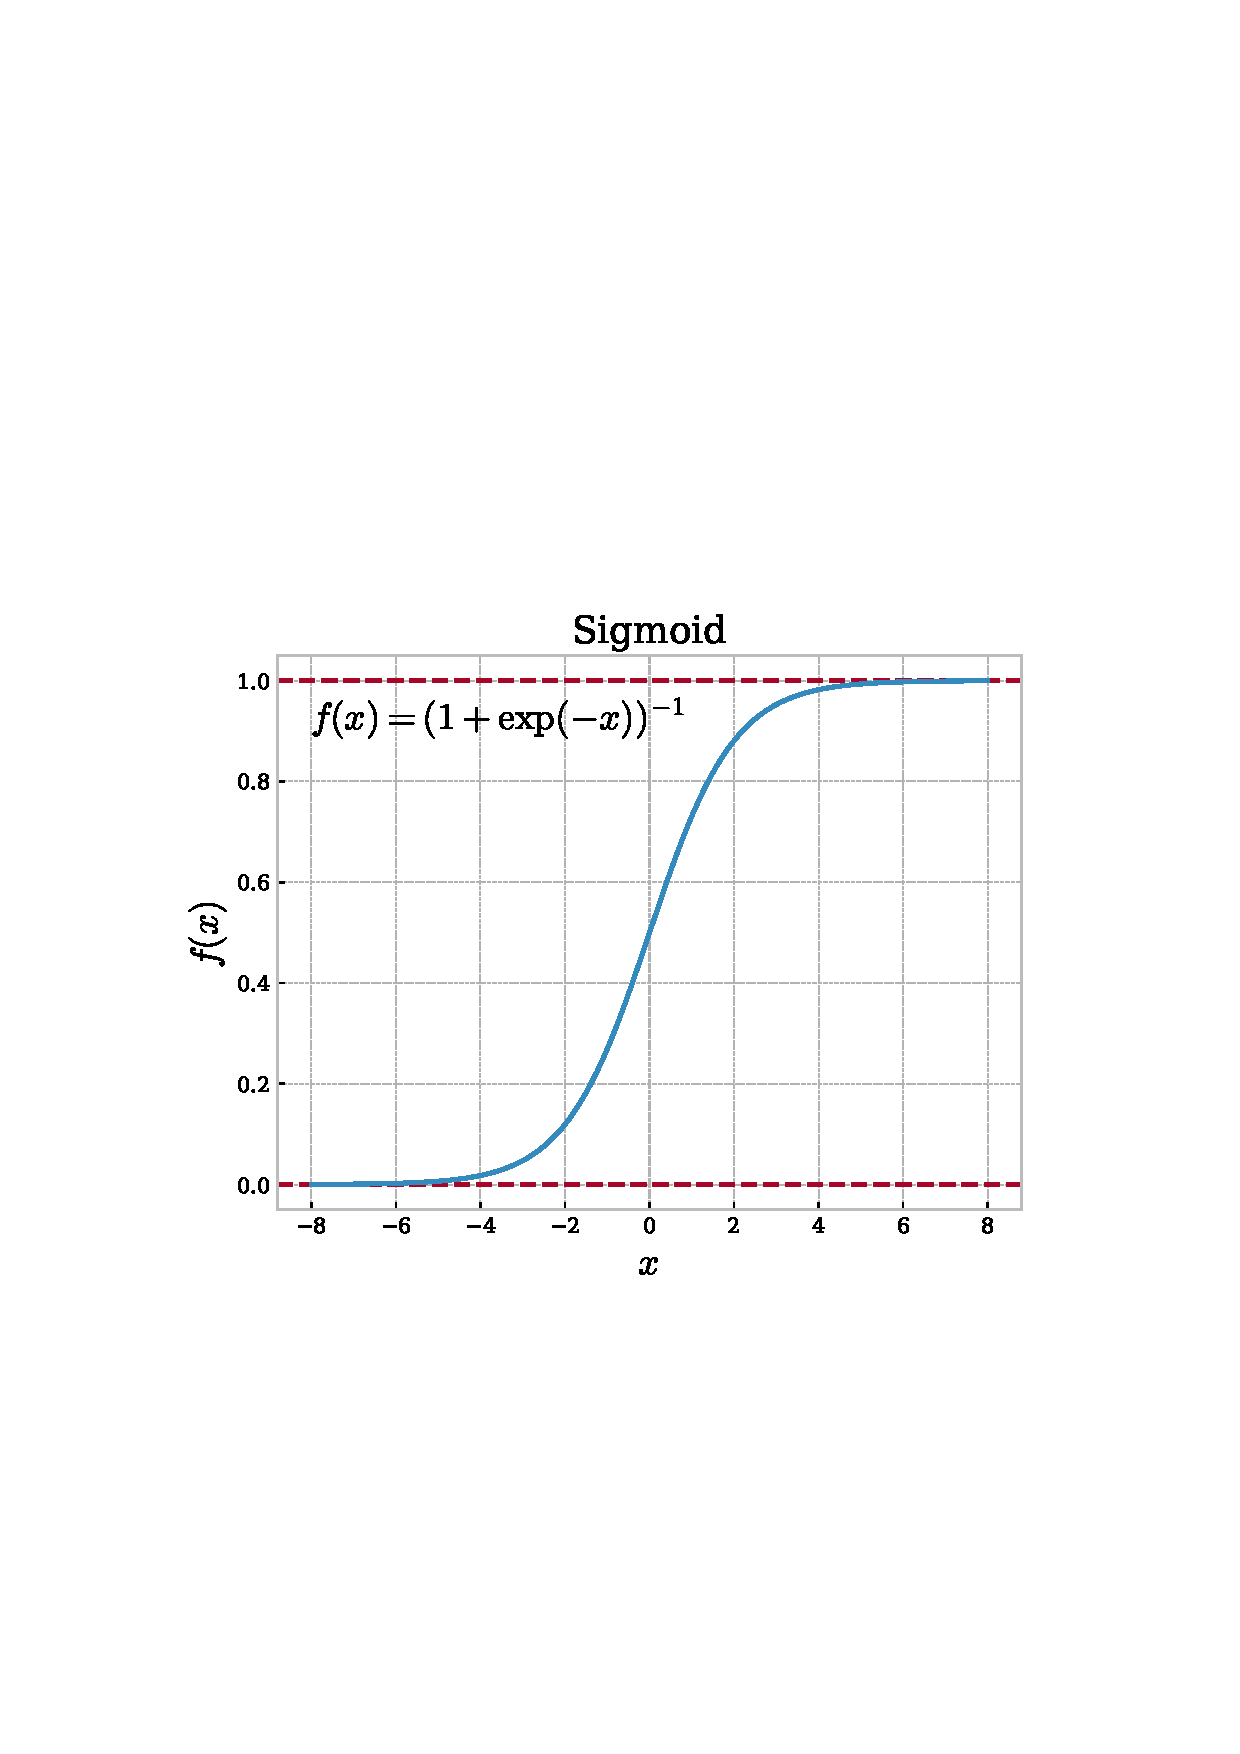
\includegraphics[width=4cm]{Images/sigmoid.png} }}
	\subfloat[ReLU]{{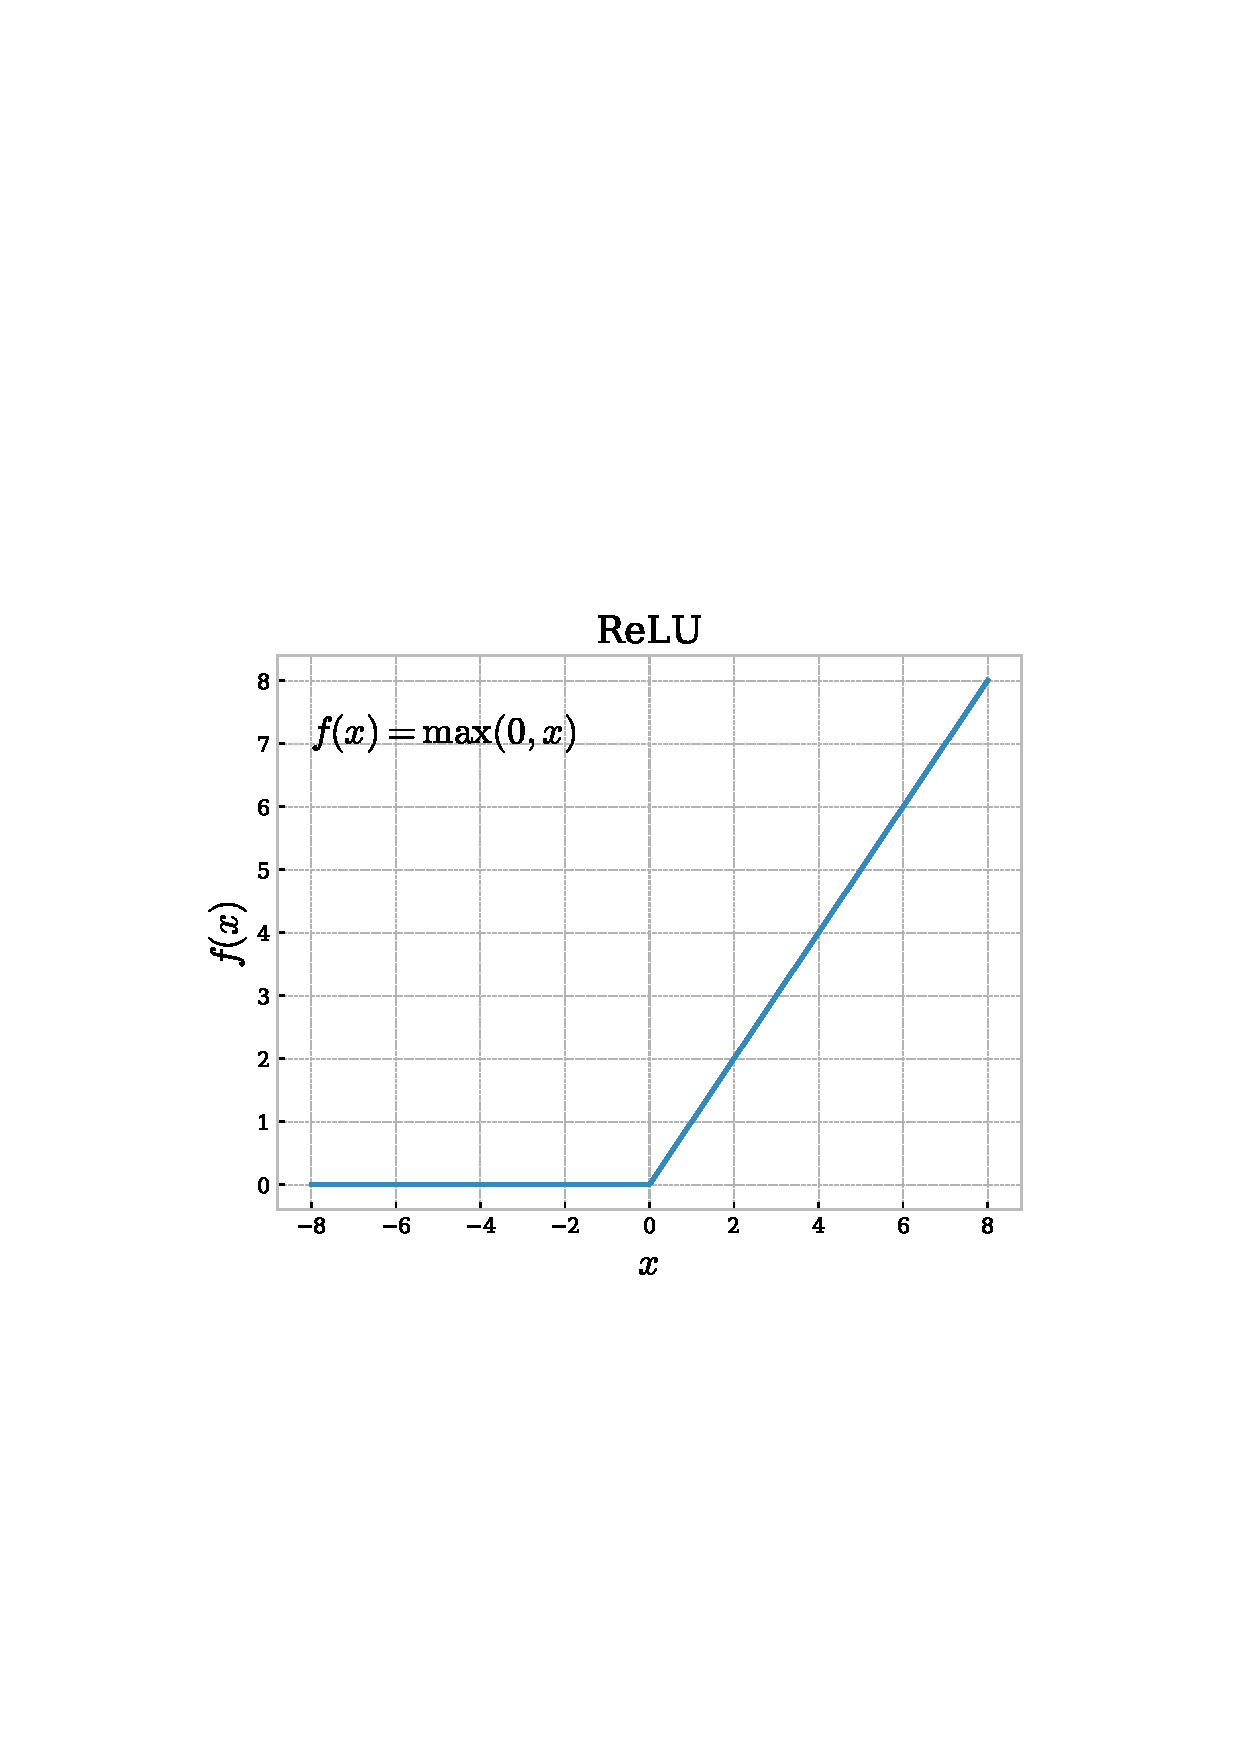
\includegraphics[width=4cm]{Images/ReLU.png}}}
	\subfloat[Leaky ReLU]{{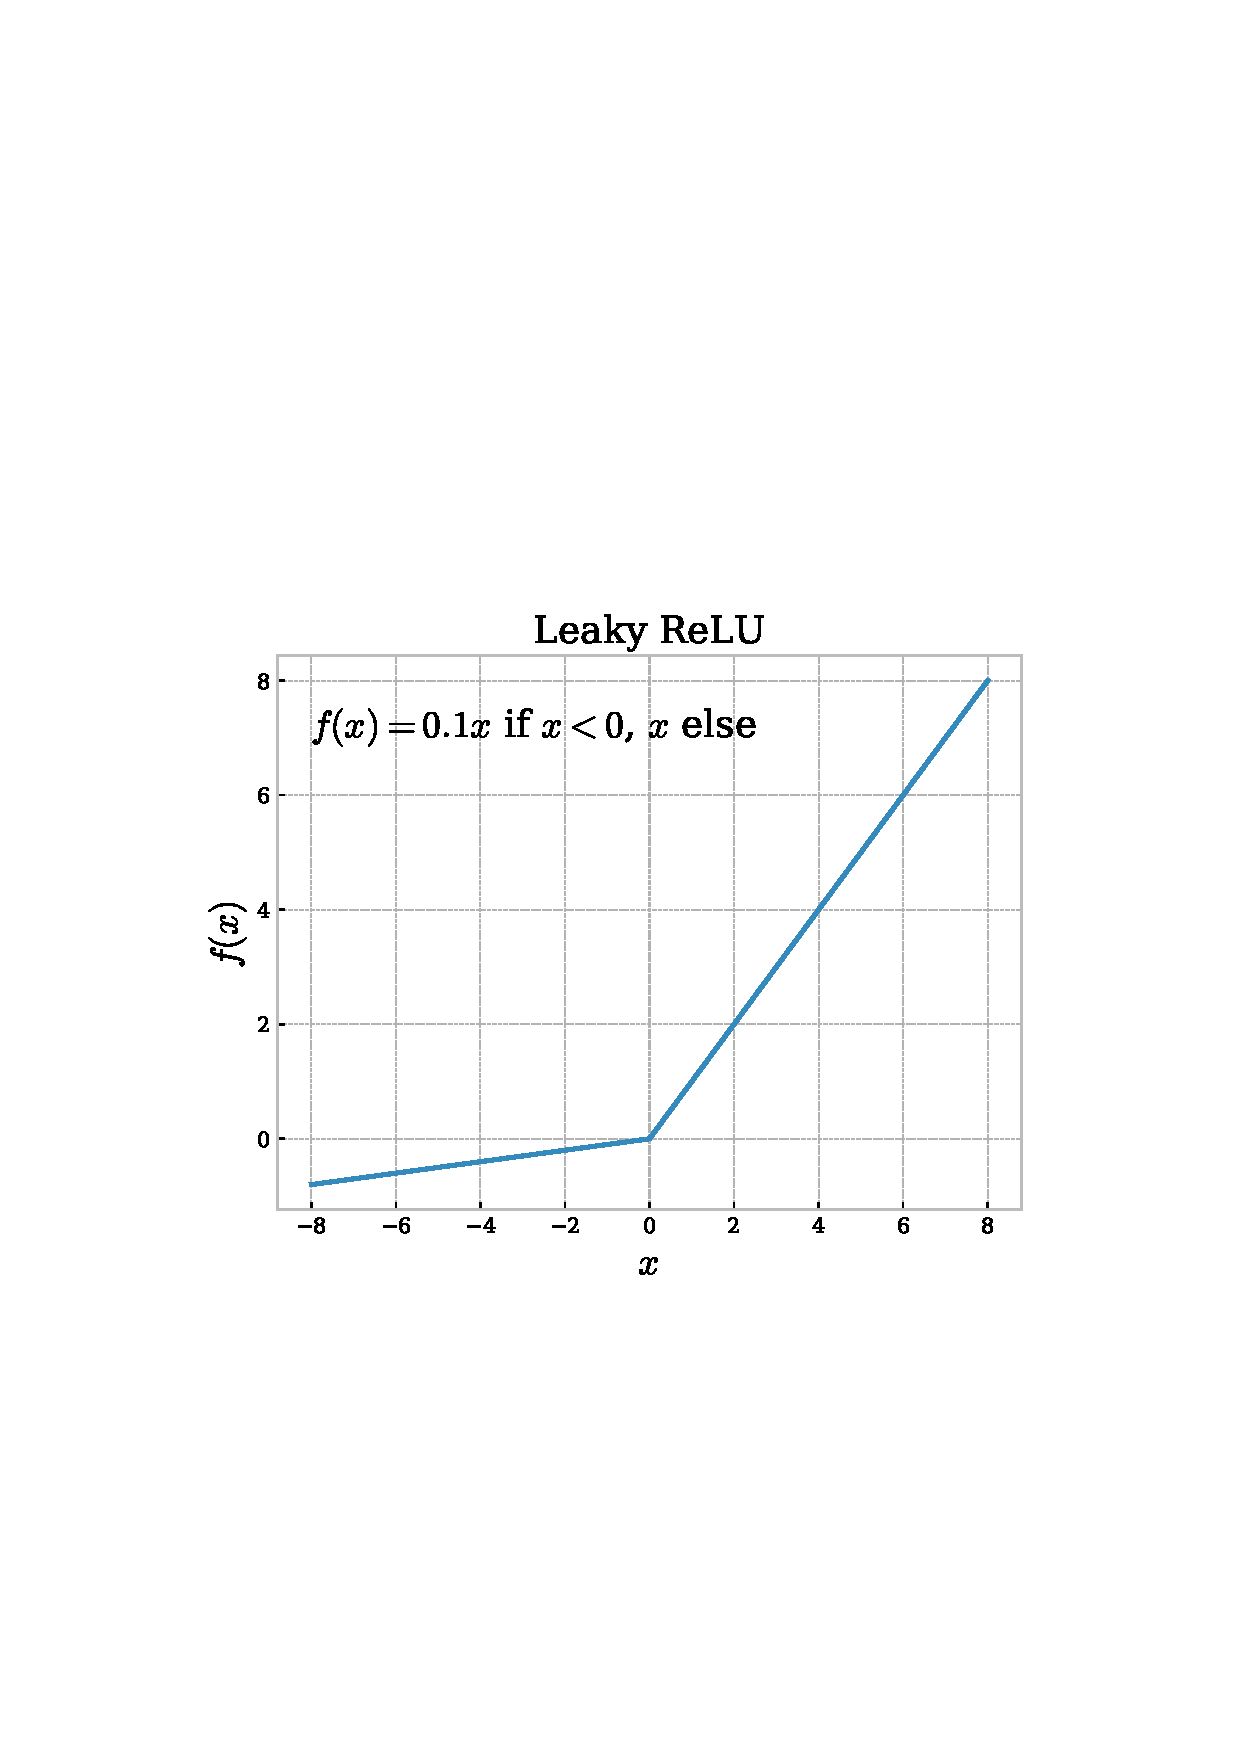
\includegraphics[width=4cm]{Images/LeakyReLU.png} }}
	\subfloat[ELU]{{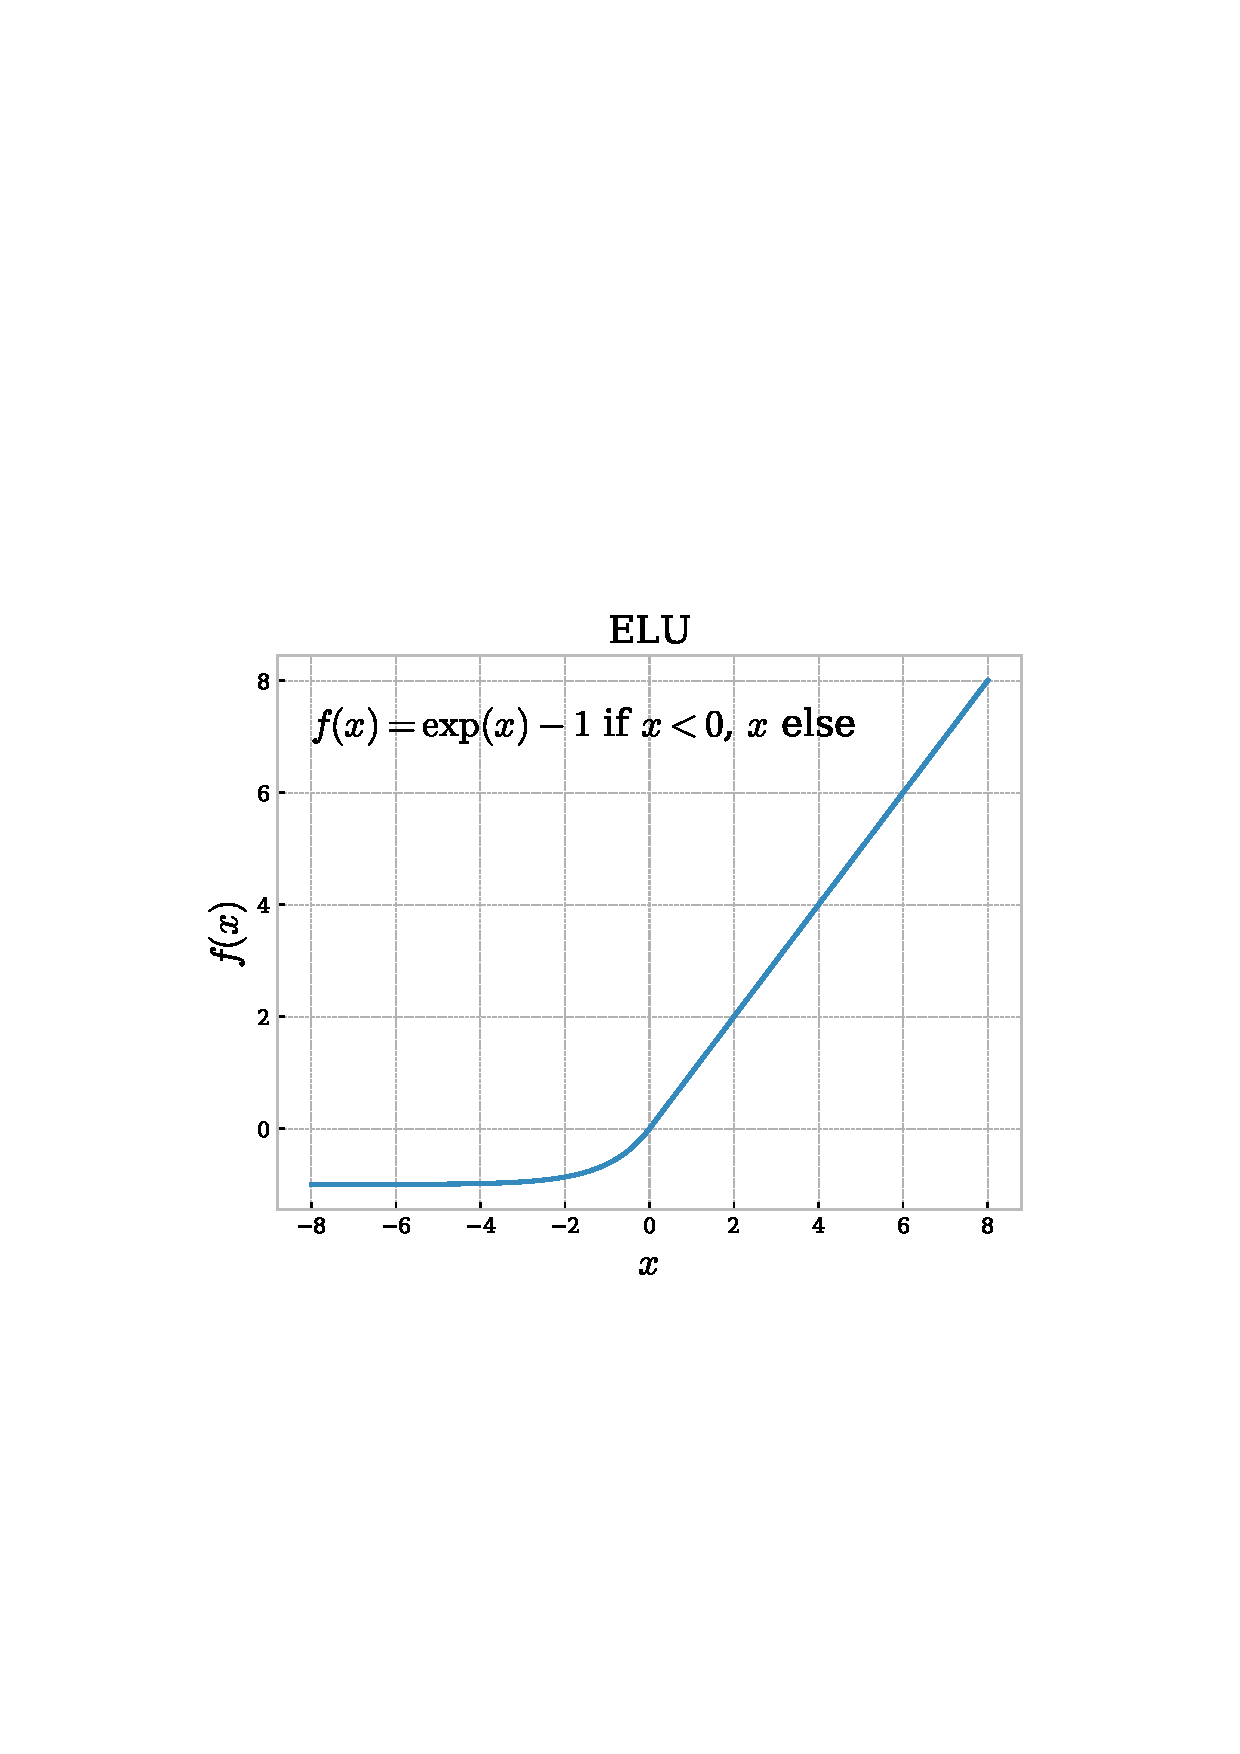
\includegraphics[width=4cm]{Images/ELU.png}}}
	\caption{Some well-known activation functions. The sigmoid function stands out from the others since it maps between 0 and 1, and it is not linear for positive numbers.}%
	\label{fig:activation_functions}%
\end{figure}


\subsubsection{Backward propagation} \label{sec:backward}
Backward propagation is the most robust technique for updating the weights in a neural network, and is actually again based on the weight update presented for linear and logistic regression. The algorithm for this was presented 1986, which made the deep neural networks able to solve relatively complicated problems for the first time \cite{rumelhart_learning_1986}. To update the weights, one starts with the outputs and updates the weights layer-wise until one gets to the inputs, hence the name backward propagation. 

As observed above, a node is dependent on all the units in the previous layers, and so are the weights. This means that the units are dependent on a large number of parameters, which makes the training scheme quite complex. Nevertheless, there is possible to generalize this to express the updating formulas on a relatively simple form.

From the linear and logistic regression, we know that we need the derivative of the cost function in order to implement the weight update regime. Again, we define the cost function as the mean square error,
\begin{equation*}
\mathcal{C}(\bs{w})=\frac{1}{2}\sum_{i=1}^{N_L}(y_i-a_i^{(L)})^2
\end{equation*}
where we have $L+1$ layers ($L$ is the last layer) and $N_L$ output units. The derivative of this with respect to one of the weights between the $L-1$'th and $L$'th layer can be written as a sum using the chain rule
\begin{equation*}
\frac{\partial\mathcal{C}(\bs{w})}{\partial w_{jk}^{(L)}}=\frac{\partial\mathcal{C}(\bs{w})}{\partial a_j^{(L)}}\frac{\partial a_j^{(L)}}{\partial z_j^{(L)}}\frac{\partial z_j^{(L)}}{\partial w_{jk}^{(L)}}.
\end{equation*}
If we start with the first factor, it can easily be found to be 
\begin{equation*}
\frac{\partial\mathcal{C}(\bs{w})}{\partial a_j^{(L)}}=(y_j-a_j^{(L)})
\end{equation*}
using the definition of the cost function. The second factor is the derivative of the activation function with respect to its argument, and is for the sigmoid function given by
\begin{equation*}
\frac{\partial a_j^{(L)}}{\partial z_j^{(L)}}=a_j^{(L)}(1-a_j^{(L)}).
\end{equation*}
Finally, the last factor is found from equation \eqref{eq:netoutput}, and we obtain
\begin{equation*}
\frac{\partial z_j^{(L)}}{\partial w_{jk}^{(L)}}=a_k^{(L-1)}.
\end{equation*}
Collecting all the factors, the last set of weights can be found by
\begin{equation*}
\frac{\partial\mathcal{C}(\bs{w})}{\partial w_{jk}^{(L)}}=(y_j-a_j^{(L)})a_j^{(L)}(1-a_j^{(L)})a_k^{(L-1)}
\end{equation*}
In the next step, we can define
\begin{equation*}
\delta_j^{(L)}=a_j^{(L)}(1-a_j^{(L)})(y_j-a_j^{(L)})=f'(a_j^{(L)})\frac{\partial \mathcal{C}(\bs{w})}{\partial a_j^{(L)}}=\frac{\partial \mathcal{C}(\bs{w})}{\partial z_j^{(L)}}
\end{equation*}
such that the weight update can be expressed on a neater form
\begin{equation*}
\frac{\partial\mathcal{C}(\bs{w})}{\partial w_{jk}^{(L)}}=\delta_j^{(L)}a_k^{(L-1)}.
\end{equation*}

For a general layer $l$, the derivative of the cost function with respect to a weight $w_{jk}^{(l)}$ is similar, and given by
\begin{empheq}[box={\mybluebox[5pt]}]{equation}
\frac{\partial\mathcal{C}(\bs{w})}{\partial w_{jk}^{(l)}}=\delta_j^{(l)}a_k^{(l-1)}.
\end{empheq}
Our goal is to find the general relation between layer $l$ and $l+1$, and therefore we use the chain rule and sum over all the net outputs in layer $l+1$,
\begin{equation*}
\delta_j^{(l)}=\frac{\partial \mathcal{C}(\bs{w})}{\partial z_j^{(l)}}=\sum_k\frac{\partial\mathcal{C}(\bs{w})}{\partial z_k^{(l+1)}}\frac{\partial z_k^{(l+1)}}{\partial z_j^{(l)}}.
\end{equation*}
We now recognize that the first factor in the sum is just $\delta_k^{(l+1)}$ and the last factor can be found from equation \eqref{eq:netoutput}. We obtain the final expression, 
\begin{empheq}[box={\mybluebox[5pt]}]{equation}
\delta_j^{(l)}=\sum_k\delta_k^{(l+1)}w_{kj}^{(l+1)}f'(z_j^{(l)})
\end{empheq}
where we use the expression of $\delta_j^{(L)}$ as our initial condition. Similar to LASSO regression, a solution of the weight update does not exist in closed form and we need to rely on interative optimization methods. Using gradient descent, a new weight $w_{ij}^{(l)+}$ is found from
\begin{empheq}[box={\mybluebox[5pt]}]{align}
w_{ij}^{(l)+}=w_{ij}^{(l)}-\eta\frac{\partial\mathcal{C}(\bs{w})}{\partial w_{jk}^{(l)}}.
\end{empheq}

\section{Optimization algorithms} \label{sec:optimizationalgorithms}
In chapter \ref{chp:machinelearning}, we discussed the gradient descent optimization algorithm, which is among the most basic methods available. That method is based on the gradient, which is the slope of the cost function, but many methods are also in need of the Hessian matrix, which gives the curvature of the cost function. We will barely scratch the surface of this field, limiting us to the gradient methods. 

To have the method fresh in mind, we will start with reintroducing the gradient descent method before we move on the its stochastic brother. We will then have a look at how momentum can be added, and finally we examine the stochastic and momentum based ADAM optimizer. 

\subsection{Gradient descent} \label{sec:gd}
Perhaps the simplest and most intuitive method for finding the minimum is the gradient descent method, which reads
\begin{empheq}[box={\mybluebox[5pt]}]{align}
\label{eq:GD}
\bs{\theta}_t=\bs{\theta}_{t-1} - \eta\nabla_{\theta} \mathcal{C}(\bs{\theta}_{t-1})
\end{empheq}
where $\bs{\theta}_t$ is the parameter vector at time step (iteration) $t$ and $\eta$ is the learning rate. $\nabla_{\theta} \mathcal{C}(\bs{\theta}_{t-1})$ is the gradient of the cost function with respect to all the parameters $\theta$ at time $t-1$. 

The idea is to find the direction where the cost function $\mathcal{C}(\bs{\theta})$ has the steepest slope, and move in the direction which minimizes the cost function. For every time step, the cost function is thus minimized, and when the gradient approaches zero the minimum is found. A possible, but basic, stop criterion is
\begin{equation}
\nabla_{\theta} \mathcal{C}(\bs{\theta}_t)<\varepsilon.
\end{equation}
where $\varepsilon$ is a tolerance. More robust methods are based on comparing the value of the cost function for several past iterations. 

In cases where the cost function is not strictly decreasing, we will have both local and global minima. Often, it is hard to say whether we are stuck in a local or global minimum, and this is where the stochasticity enters the game.

\subsection{Stochastic gradient descent}\label{sec:sgd}
Stochastic gradient descent is closely related to the gradient descent method, but the method uses randomly selected batches to evaluate the gradients, hence the stochasticity. By introducing this randomness, the parameters will not always be updated in order to minimize the energy, which makes us less likely to be stuck in a local minimum.

In practice, one splits the data set in $n$ batches, and select one of them to be used in the parameter update. Our hope is that this batch is representative for the entire data set, such that the new parameters gives a lower cost function. If that is the case, we have reduced the cost of an iteration significantly, since we only need to care about a batch. After each batch in the data set has had an opportunity to update the internal parameters, we say that we have went through an \textit{epoch}.

We are not guaranteed that updating the parameters with respect to a batch gives a lower cost function, and when it is not, we need to run more batches in order to minimize the cost function. Since each iteration is faster than for standard gradient descent, this is acceptable. As long as the batch is slightly representative for the entire data set, the cost function will be minimized in the end.

Mathematically, the method can be expressed as 
\begin{empheq}[box={\mybluebox[5pt]}]{align}
\label{eq:SGD}
\bs{\theta}_t=\bs{\theta}_{t-1} - \eta\nabla_{\theta} \mathcal{C}_i(\bs{\theta}_{t-1})
\end{empheq}
where we use the $i$'th batch in the parameter update. Standard gradient descent is actually just a special case of this, where we only have one batch ($i$ includes the whole data set). If we still get stuck in local minima after adding the stochasticity, it might be a good idea to add momentum as well.

\subsection{Adding momentum} \label{sec:momentum}
If we go back to an introductory mechanics course, you might remember that momentum is a quantity that maintains the motion of a body. Imagine a ball that rolls down a steep hill, but then there is a local minimum that it needs to escape to keep rolling. If it has enough momentum, it will be able to escape.

Exactly the same idea lies behind the momentum used in optimization algorithms; the momentum will try to maintain the motion towards the global minimum, which makes the system less likely to be stuck in a local minimum.  

Momentum can be added to most optimization algorithms, also gradient descent and stochastic gradient descent. The way we do it is to save the direction we were moving in the previous iteration, and use it as a contribution to the next gradient update. A typical implementation of the first-order momentum looks like
\begin{empheq}[box={\mybluebox[5pt]}]{equation}
\begin{aligned}
\bs{m}_t &= \gamma\bs{m}_{t-1} + \eta\nabla_{\theta} \mathcal{C}_i(\bs{\theta}_{t-1})\\
\bs{\theta}_t&=\bs{\theta}_{t-1}-\bs{m}_t
\end{aligned}
\end{empheq}
where $\gamma$ is the momentum parameter, which is just another hyper-parameter usually initialized to a small number. $\bs{m}_t$ is the momentum vector, and can be initialized as the zero vector.

The optimization algorithm can be modified further in unlimited ways. A common improvement is to add higher order momentum, another is to make the learning rate adaptive. We have implemented the most basic version of this, with monotonic adaptivity. Many algorithms, such as the conjugate gradient method, also make use of the Hessian as discussed in the introduction, but that is another level of complexity. 

We will end this section with setting up the algorithm of a stochastic gradient descent optimization with momentum and monotonic adaptivity. The algorithm is found in algorithm \eqref{alg:asgd}.

\IncMargin{1em}
\begin{algorithm}
	\SetAlgoLined
	\Parameter{$\eta$: Learning rate}
	\Parameter{$\gamma$: Momentum parameter}
	\Parameter{$\lambda$: Monotonic decay rate}
	\Require{$\mathcal{C}(\bs{\theta})$: Cost function}
	\Data{$\bs{\theta}_0$: Initial parameters}
	
	$\bs{m}_0\leftarrow 0$ (Initialize momentum vector)\;
	$t\leftarrow 0$ (Initialize time step)\;
	\While{$\bs{\theta}_t$ not converged}{
		$t\leftarrow t+1$ (Increase time for each iteration)\;
		$\bs{g}_t\leftarrow \nabla_{\theta}\mathcal{C}_t(\bs{\theta}_{t-1})$ (Get gradients from a given batch at time $t$)\;
		$\bs{m}_t\leftarrow \gamma\bs{m}_{t-1}+\eta\cdot\bs{g}_t$ (Update first momentum estimate)\;
		$\bs{\theta}_t=\bs{\theta}_{t-1}-\eta\cdot\bs{m}_t/\lambda^t$ (Update parameters)\;
	}
	\KwResult{Updated parameters $\bs{\theta}_t$ after convergence}
	\caption{Adaptive stochastic gradient descent with momentum. See sections (\ref{sec:sgd}-\ref{sec:momentum}) for details. Robust default settings for the hyper-parameters are $\eta=0.001$, $\gamma=0.01$ and $\lambda=0.1$. All the operations are element-wise.}
	\label{alg:asgd}
\end{algorithm}\DecMargin{1em}

\subsection{ADAM} \label{sec:adam}
ADAM is a first-order stochastic optimization method which is widely used in machine learning. It was discovered by D.P. Kingma and J. Ba, and published in a 2014 paper. The article has already more than 25000 citations! \cite{kingma_adam:_2014} So what makes this method so popular? 

The main reason why it is widely used, is obviously that it performs good. The fact that it only requires the gradient makes it efficient, and the way the momentum is implemented still makes able to handle a large number of parameters. 

The optimization algorithm can be expressed as a set of equations
\begin{empheq}[box={\mybluebox[5pt]}]{equation}
\begin{aligned}
\bs{g}_t&=\nabla_{\theta} \mathcal{C}_t(\bs{\theta}_{t-1})\\
\bs{m}_t&=\gamma_1\bs{m}_{t-1}+(1-\gamma_1)\bs{g}_t\\
\bs{v}_t&=\gamma_2\bs{v}_{t-1}+(1-\gamma_2)\bs{g}_t^2\\
\hat{\bs{m}}_t&=\bs{m}_t/(1-\gamma_1^t)\\
\hat{\bs{v}}_t&=\bs{v}_t/(1-\gamma_2^t)\\
\bs{\theta}_t&=\bs{\theta}_{t-1}-\eta\hat{\bs{m}}_t/(\sqrt{\hat{\bs{v}}_t}+\bs{\varepsilon})
\end{aligned}
\end{empheq}
where $\bs{m}_t$ is the biased first momentum estimate of the parameter vector $\bs{\theta}$ and $\bs{v}_t$ is the biased second raw moment estimate. The momentum parameters need to be in the range $\gamma_1,\gamma_2\in[0,1)$, and are often set to values close to 1. This makes the optimization adaptive: as time goes, the factors $1-\gamma_1^t$ and $1-\gamma_2^t$ approach 1 from below. $\eta$ corresponds to the learning rate, and should be a small number. Finally, the parameter $\varepsilon$ is added to avoid division by zero. 

We can set up the algorithm in a similar manner to the adaptive stochastic gradient descent algorithm from above, which gives the algorithm \eqref{alg:adam}.

\IncMargin{1em}
\begin{algorithm}
	\SetAlgoLined
	\Parameter{$\eta$: Learning rate}
	\Parameter{$\gamma_1,\gamma_2\in [0,1)$: Momentum parameters}
	\Parameter{$\varepsilon$: Division parameter}
	\Require{$\mathcal{C}(\bs{\theta})$: Cost function}
	\Data{$\bs{\theta}_0$: Initial parameters}
	
	$\bs{m}_0\leftarrow 0$ (Initialize 1$^{\text{st}}$ momentum vector)\;
	$\bs{v}_0\leftarrow 0$ (Initialize 2$^{\text{st}}$ momentum vector)\;
	$t\leftarrow 0$ (Initialize time step)\;
	\While{$\bs{\theta}_t$ not converged}{
		$t\leftarrow t+1$ (Increase time for each iteration)\;
		$\bs{g}_t\leftarrow \nabla_{\theta}\mathcal{C}_t(\bs{\theta}_{t-1})$ (Get gradients from a given batch at time $t$)\;
		$\bs{m}_t\leftarrow \gamma_1\bs{m}_{t-1}+(1-\gamma_1)\cdot\bs{g}_t$ (Update first momentum estimate)\;
		$\bs{v}_t\leftarrow \gamma_2\bs{v}_{t-1}+(1-\gamma_2)\cdot\bs{g}_t^2$ (Update second raw momentum estimate)\;
		$\hat{\bs{m}}_t\leftarrow\bs{m}_t/(1-\gamma_1^t)$ (Bias-corrected first momentum estimate)\;
		$\hat{\bs{v}}_t\leftarrow\bs{v}_t/(1-\gamma_2^t)$ (Bias-corrected second momentum estimate) \;
		$\bs{\theta}_t\leftarrow\bs{\theta}_{t-1}-\eta\cdot\hat{\bs{m}}_t/(\sqrt{\hat{\bs{v}}_t}+\bs{\varepsilon})$ (Update parameters) \;
	}
	\KwResult{Updated parameters $\bs{\theta}_t$ after convergence}
	\caption{ADAM optimizer. Robust default settings for the hyper-parameters are $\eta=0.001$, $\gamma=0.01$ and $\lambda=0.1$. All the operations are element-wise, and for in-depth information see the original paper, \cite{kingma_adam:_2014}.}
	\label{alg:adam}
\end{algorithm}\DecMargin{1em}